\documentclass[twoside]{book}

% Packages required by doxygen
\usepackage{fixltx2e}
\usepackage{calc}
\usepackage{doxygen}
\usepackage[export]{adjustbox} % also loads graphicx
\usepackage{graphicx}
\usepackage[utf8]{inputenc}
\usepackage{makeidx}
\usepackage{multicol}
\usepackage{multirow}
\PassOptionsToPackage{warn}{textcomp}
\usepackage{textcomp}
\usepackage[nointegrals]{wasysym}
\usepackage[table]{xcolor}

% Font selection
\usepackage[T1]{fontenc}
\usepackage[scaled=.90]{helvet}
\usepackage{courier}
\usepackage{amssymb}
\usepackage{sectsty}
\renewcommand{\familydefault}{\sfdefault}
\allsectionsfont{%
  \fontseries{bc}\selectfont%
  \color{darkgray}%
}
\renewcommand{\DoxyLabelFont}{%
  \fontseries{bc}\selectfont%
  \color{darkgray}%
}
\newcommand{\+}{\discretionary{\mbox{\scriptsize$\hookleftarrow$}}{}{}}

% Page & text layout
\usepackage{geometry}
\geometry{%
  a4paper,%
  top=2.5cm,%
  bottom=2.5cm,%
  left=2.5cm,%
  right=2.5cm%
}
\tolerance=750
\hfuzz=15pt
\hbadness=750
\setlength{\emergencystretch}{15pt}
\setlength{\parindent}{0cm}
\setlength{\parskip}{3ex plus 2ex minus 2ex}
\makeatletter
\renewcommand{\paragraph}{%
  \@startsection{paragraph}{4}{0ex}{-1.0ex}{1.0ex}{%
    \normalfont\normalsize\bfseries\SS@parafont%
  }%
}
\renewcommand{\subparagraph}{%
  \@startsection{subparagraph}{5}{0ex}{-1.0ex}{1.0ex}{%
    \normalfont\normalsize\bfseries\SS@subparafont%
  }%
}
\makeatother

% Headers & footers
\usepackage{fancyhdr}
\pagestyle{fancyplain}
\fancyhead[LE]{\fancyplain{}{\bfseries\thepage}}
\fancyhead[CE]{\fancyplain{}{}}
\fancyhead[RE]{\fancyplain{}{\bfseries\leftmark}}
\fancyhead[LO]{\fancyplain{}{\bfseries\rightmark}}
\fancyhead[CO]{\fancyplain{}{}}
\fancyhead[RO]{\fancyplain{}{\bfseries\thepage}}
\fancyfoot[LE]{\fancyplain{}{}}
\fancyfoot[CE]{\fancyplain{}{}}
\fancyfoot[RE]{\fancyplain{}{\bfseries\scriptsize Generated by Doxygen }}
\fancyfoot[LO]{\fancyplain{}{\bfseries\scriptsize Generated by Doxygen }}
\fancyfoot[CO]{\fancyplain{}{}}
\fancyfoot[RO]{\fancyplain{}{}}
\renewcommand{\footrulewidth}{0.4pt}
\renewcommand{\chaptermark}[1]{%
  \markboth{#1}{}%
}
\renewcommand{\sectionmark}[1]{%
  \markright{\thesection\ #1}%
}

% Indices & bibliography
\usepackage{natbib}
\usepackage[titles]{tocloft}
\setcounter{tocdepth}{3}
\setcounter{secnumdepth}{5}
\makeindex

% Hyperlinks (required, but should be loaded last)
\usepackage{ifpdf}
\ifpdf
  \usepackage[pdftex,pagebackref=true]{hyperref}
\else
  \usepackage[ps2pdf,pagebackref=true]{hyperref}
\fi
\hypersetup{%
  colorlinks=true,%
  linkcolor=blue,%
  citecolor=blue,%
  unicode%
}

% Custom commands
\newcommand{\clearemptydoublepage}{%
  \newpage{\pagestyle{empty}\cleardoublepage}%
}

\usepackage{caption}
\captionsetup{labelsep=space,justification=centering,font={bf},singlelinecheck=off,skip=4pt,position=top}

%===== C O N T E N T S =====

\begin{document}

% Titlepage & ToC
\hypersetup{pageanchor=false,
             bookmarksnumbered=true,
             pdfencoding=unicode
            }
\pagenumbering{roman}
\begin{titlepage}
\vspace*{7cm}
\begin{center}%
{\Large My Project }\\
\vspace*{1cm}
{\large Generated by Doxygen 1.8.11}\\
\end{center}
\end{titlepage}
\clearemptydoublepage
\tableofcontents
\clearemptydoublepage
\pagenumbering{arabic}
\hypersetup{pageanchor=true}

%--- Begin generated contents ---
\chapter{File Index}
\section{File List}
Here is a list of all files with brief descriptions\+:\begin{DoxyCompactList}
\item\contentsline{section}{\hyperlink{Lab1_8c}{Lab1.\+c} }{\pageref{Lab1_8c}}{}
\end{DoxyCompactList}

\chapter{File Documentation}
\hypertarget{WireLength_8cpp}{}\section{Wire\+Length.\+cpp File Reference}
\label{WireLength_8cpp}\index{Wire\+Length.\+cpp@{Wire\+Length.\+cpp}}
{\ttfamily \#include $<$stdio.\+h$>$}\\*
{\ttfamily \#include $<$limits.\+h$>$}\\*
{\ttfamily \#include $<$iostream$>$}\\*
Include dependency graph for Wire\+Length.\+cpp\+:
\nopagebreak
\begin{figure}[H]
\begin{center}
\leavevmode
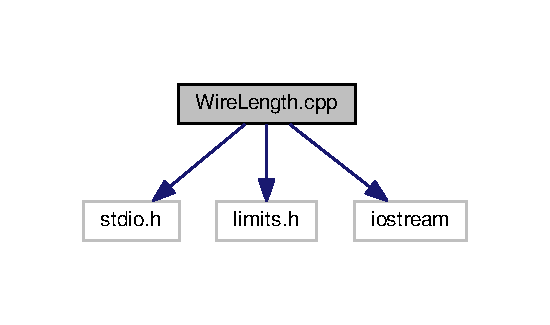
\includegraphics[width=264pt]{WireLength_8cpp__incl}
\end{center}
\end{figure}
\subsection*{Macros}
\begin{DoxyCompactItemize}
\item 
\#define \hyperlink{WireLength_8cpp_af40a326b23c68a27cebe60f16634a2cb}{V}~9
\end{DoxyCompactItemize}
\subsection*{Functions}
\begin{DoxyCompactItemize}
\item 
int \hyperlink{WireLength_8cpp_abba4f89d0af30ad867c4af65994356e6}{min\+Distance} (int dist\mbox{[}$\,$\mbox{]}, bool spt\+Set\mbox{[}$\,$\mbox{]})
\item 
void \hyperlink{WireLength_8cpp_ae3e29823807c3e9a84c4f3dfe59b5706}{print\+Solution} (int dist\mbox{[}$\,$\mbox{]}, int n)
\item 
void \hyperlink{WireLength_8cpp_a4f3e5793caae32aeb0d5482f45865c5b}{optimize\+Length} (int graph\mbox{[}\hyperlink{WireLength_8cpp_af40a326b23c68a27cebe60f16634a2cb}{V}\mbox{]}\mbox{[}\hyperlink{WireLength_8cpp_af40a326b23c68a27cebe60f16634a2cb}{V}\mbox{]}, int src)
\item 
int \hyperlink{WireLength_8cpp_ae66f6b31b5ad750f1fe042a706a4e3d4}{main} ()
\end{DoxyCompactItemize}


\subsection{Macro Definition Documentation}
\index{Wire\+Length.\+cpp@{Wire\+Length.\+cpp}!V@{V}}
\index{V@{V}!Wire\+Length.\+cpp@{Wire\+Length.\+cpp}}
\subsubsection[{\texorpdfstring{V}{V}}]{\setlength{\rightskip}{0pt plus 5cm}\#define V~9}\hypertarget{WireLength_8cpp_af40a326b23c68a27cebe60f16634a2cb}{}\label{WireLength_8cpp_af40a326b23c68a27cebe60f16634a2cb}


\subsection{Function Documentation}
\index{Wire\+Length.\+cpp@{Wire\+Length.\+cpp}!main@{main}}
\index{main@{main}!Wire\+Length.\+cpp@{Wire\+Length.\+cpp}}
\subsubsection[{\texorpdfstring{main()}{main()}}]{\setlength{\rightskip}{0pt plus 5cm}int main (
\begin{DoxyParamCaption}
{}
\end{DoxyParamCaption}
)}\hypertarget{WireLength_8cpp_ae66f6b31b5ad750f1fe042a706a4e3d4}{}\label{WireLength_8cpp_ae66f6b31b5ad750f1fe042a706a4e3d4}

\begin{DoxyCode}
76 \{
77     \textcolor{comment}{/* Let us create the example graph discussed above */}
78     \textcolor{keywordtype}{int} graph[\hyperlink{WireLength_8cpp_af40a326b23c68a27cebe60f16634a2cb}{V}][\hyperlink{WireLength_8cpp_af40a326b23c68a27cebe60f16634a2cb}{V}] =
79             \{ \{ 0, 4, 0, 0, 0, 0, 0, 8, 0 \}, \{ 4, 0, 8, 0, 0, 0, 0, 11, 0 \}, \{
80                     0, 8, 0, 7, 0, 4, 0, 0, 2 \},
81                     \{ 0, 0, 7, 0, 9, 14, 0, 0, 0 \}, \{ 0, 0, 0, 9, 0, 10, 0, 0,
82                             0 \}, \{ 0, 0, 4, 0, 10, 0, 2, 0, 0 \}, \{ 0, 0, 0, 14,
83                             0, 2, 0, 1, 6 \}, \{ 8, 11, 0, 0, 0, 0, 1, 0, 7 \}, \{
84                             0, 0, 2, 0, 0, 0, 6, 7, 0 \} \};
85  
86     cout << \textcolor{stringliteral}{"Enter the starting component: "};
87     \textcolor{keywordtype}{int} s;
88     cin >> s;
89     \hyperlink{WireLength_8cpp_a4f3e5793caae32aeb0d5482f45865c5b}{optimizeLength}(graph, s);
90  
91     \textcolor{keywordflow}{return} 0;
92 \}\end{DoxyCode}


Here is the call graph for this function\+:
\nopagebreak
\begin{figure}[H]
\begin{center}
\leavevmode
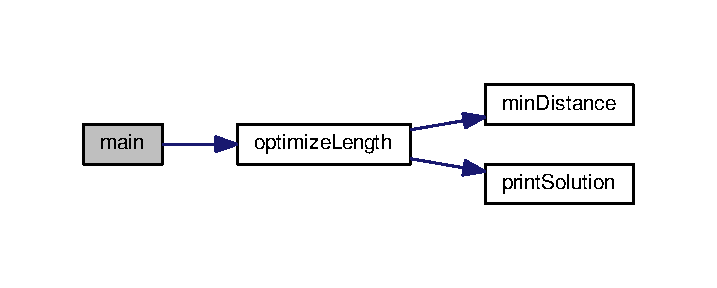
\includegraphics[width=344pt]{WireLength_8cpp_ae66f6b31b5ad750f1fe042a706a4e3d4_cgraph}
\end{center}
\end{figure}


\index{Wire\+Length.\+cpp@{Wire\+Length.\+cpp}!min\+Distance@{min\+Distance}}
\index{min\+Distance@{min\+Distance}!Wire\+Length.\+cpp@{Wire\+Length.\+cpp}}
\subsubsection[{\texorpdfstring{min\+Distance(int dist[], bool spt\+Set[])}{minDistance(int dist[], bool sptSet[])}}]{\setlength{\rightskip}{0pt plus 5cm}int min\+Distance (
\begin{DoxyParamCaption}
\item[{int}]{dist\mbox{[}$\,$\mbox{]}, }
\item[{bool}]{spt\+Set\mbox{[}$\,$\mbox{]}}
\end{DoxyParamCaption}
)}\hypertarget{WireLength_8cpp_abba4f89d0af30ad867c4af65994356e6}{}\label{WireLength_8cpp_abba4f89d0af30ad867c4af65994356e6}

\begin{DoxyCode}
13 \{
14     \textcolor{comment}{// Initialize min value}
15     \textcolor{keywordtype}{int} min = INT\_MAX, min\_index;
16  
17     \textcolor{keywordflow}{for} (\textcolor{keywordtype}{int} v = 0; v < \hyperlink{WireLength_8cpp_af40a326b23c68a27cebe60f16634a2cb}{V}; v++)
18         \textcolor{keywordflow}{if} (sptSet[v] == \textcolor{keyword}{false} && dist[v] <= min)
19             min = dist[v], min\_index = v;
20  
21     \textcolor{keywordflow}{return} min\_index;
22 \}
\end{DoxyCode}
\index{Wire\+Length.\+cpp@{Wire\+Length.\+cpp}!optimize\+Length@{optimize\+Length}}
\index{optimize\+Length@{optimize\+Length}!Wire\+Length.\+cpp@{Wire\+Length.\+cpp}}
\subsubsection[{\texorpdfstring{optimize\+Length(int graph[V][V], int src)}{optimizeLength(int graph[V][V], int src)}}]{\setlength{\rightskip}{0pt plus 5cm}void optimize\+Length (
\begin{DoxyParamCaption}
\item[{int}]{graph\mbox{[}\+V\mbox{]}\mbox{[}\+V\mbox{]}, }
\item[{int}]{src}
\end{DoxyParamCaption}
)}\hypertarget{WireLength_8cpp_a4f3e5793caae32aeb0d5482f45865c5b}{}\label{WireLength_8cpp_a4f3e5793caae32aeb0d5482f45865c5b}

\begin{DoxyCode}
35 \{
36     \textcolor{keywordtype}{int} dist[\hyperlink{WireLength_8cpp_af40a326b23c68a27cebe60f16634a2cb}{V}]; \textcolor{comment}{// The output array.  dist[i] will hold the shortest}
37     \textcolor{comment}{// distance from src to i}
38  
39     \textcolor{keywordtype}{bool} sptSet[\hyperlink{WireLength_8cpp_af40a326b23c68a27cebe60f16634a2cb}{V}]; \textcolor{comment}{// sptSet[i] will true if component i is included in shortest}
40     \textcolor{comment}{// path tree or shortest distance from src to i is finalized}
41  
42     \textcolor{comment}{// Initialize all distances as INFINITE and stpSet[] as false}
43     \textcolor{keywordflow}{for} (\textcolor{keywordtype}{int} i = 0; i < \hyperlink{WireLength_8cpp_af40a326b23c68a27cebe60f16634a2cb}{V}; i++)
44         dist[i] = INT\_MAX, sptSet[i] = \textcolor{keyword}{false};
45  
46     \textcolor{comment}{// Distance of source component from itself is always 0}
47     dist[src] = 0;
48  
49     \textcolor{comment}{// Find shortest path for all components}
50     \textcolor{keywordflow}{for} (\textcolor{keywordtype}{int} count = 0; count < V - 1; count++)
51     \{
52         \textcolor{comment}{// Pick the minimum distance component from the set of components not}
53         \textcolor{comment}{// yet processed. u is always equal to src in first iteration.}
54         \textcolor{keywordtype}{int} u = \hyperlink{WireLength_8cpp_abba4f89d0af30ad867c4af65994356e6}{minDistance}(dist, sptSet);
55  
56         \textcolor{comment}{// Mark the picked component as processed}
57         sptSet[u] = \textcolor{keyword}{true};
58  
59         \textcolor{comment}{// Update dist value of the adjacent components of the picked component.}
60         \textcolor{keywordflow}{for} (\textcolor{keywordtype}{int} v = 0; v < \hyperlink{WireLength_8cpp_af40a326b23c68a27cebe60f16634a2cb}{V}; v++)
61  
62             \textcolor{comment}{// Update dist[v] only if is not in sptSet, there is an edge from}
63             \textcolor{comment}{// u to v, and total weight of path from src to  v through u is}
64             \textcolor{comment}{// smaller than current value of dist[v]}
65             \textcolor{keywordflow}{if} (!sptSet[v] && graph[u][v] && dist[u] != INT\_MAX && dist[u]
66                     + graph[u][v] < dist[v])
67                 dist[v] = dist[u] + graph[u][v];
68     \}
69  
70     \textcolor{comment}{// print the constructed distance array}
71     \hyperlink{WireLength_8cpp_ae3e29823807c3e9a84c4f3dfe59b5706}{printSolution}(dist, V);
72 \}
\end{DoxyCode}


Here is the call graph for this function\+:
\nopagebreak
\begin{figure}[H]
\begin{center}
\leavevmode
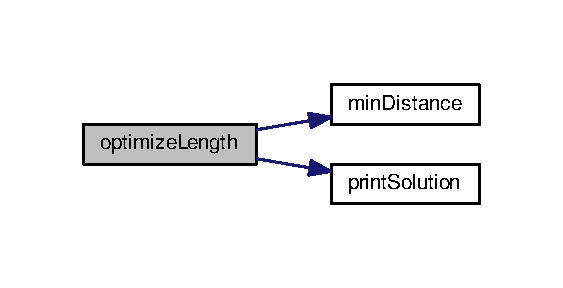
\includegraphics[width=270pt]{WireLength_8cpp_a4f3e5793caae32aeb0d5482f45865c5b_cgraph}
\end{center}
\end{figure}


\index{Wire\+Length.\+cpp@{Wire\+Length.\+cpp}!print\+Solution@{print\+Solution}}
\index{print\+Solution@{print\+Solution}!Wire\+Length.\+cpp@{Wire\+Length.\+cpp}}
\subsubsection[{\texorpdfstring{print\+Solution(int dist[], int n)}{printSolution(int dist[], int n)}}]{\setlength{\rightskip}{0pt plus 5cm}void print\+Solution (
\begin{DoxyParamCaption}
\item[{int}]{dist\mbox{[}$\,$\mbox{]}, }
\item[{int}]{n}
\end{DoxyParamCaption}
)}\hypertarget{WireLength_8cpp_ae3e29823807c3e9a84c4f3dfe59b5706}{}\label{WireLength_8cpp_ae3e29823807c3e9a84c4f3dfe59b5706}

\begin{DoxyCode}
26 \{
27     cout << \textcolor{stringliteral}{"Component\(\backslash\)tDistance from other component\(\backslash\)n"};
28     \textcolor{keywordflow}{for} (\textcolor{keywordtype}{int} i = 0; i < \hyperlink{WireLength_8cpp_af40a326b23c68a27cebe60f16634a2cb}{V}; i++)
29         printf(\textcolor{stringliteral}{"%d\(\backslash\)t\(\backslash\)t%d\(\backslash\)n"}, i, dist[i]);
30 \}
\end{DoxyCode}

%--- End generated contents ---

% Index
\backmatter
\newpage
\phantomsection
\clearemptydoublepage
\addcontentsline{toc}{chapter}{Index}
\printindex

\end{document}
